\documentclass[12pt,titlepage]{article}
\usepackage[margin=1.25in]{geometry}
\usepackage{graphicx,amsmath,minted}

%% Variables definition
\newcommand{\vSubject}{Database}
\newcommand{\vSubtitle}{Final Project - Room Tenant System}
\newcommand{\vName}{Dicha Zelianivan Arkana}
\newcommand{\vNIM}{2241720002}
\newcommand{\vClass}{1i}
\newcommand{\vDepartment}{Information Technology}
\newcommand{\vStudyProgram}{D4 Informatics Engineering}

%% [START] Tikz related stuff
\usepackage{tikz}
\usetikzlibrary{svg.path,calc,shapes.geometric,shapes.misc}
\tikzstyle{terminator} = [rectangle, draw, text centered, rounded corners = 1em, minimum height=2em]
\tikzstyle{preparation} = [chamfered rectangle, chamfered rectangle sep=0.75em, draw, text centered, minimum height = 2em]
\tikzstyle{process} = [rectangle, draw, text centered, minimum height=2em]
\tikzstyle{decision} = [diamond, aspect=2, draw, text centered, minimum height=2em]
\tikzstyle{data}=[trapezium, draw, text centered, trapezium left angle=60, trapezium right angle=120, minimum height=2em]
\tikzstyle{connector} = [line width=0.25mm,->]
%% [END] Tikz related stuff

%% [START] Fancy header related stuff
\usepackage{fancyhdr}
\pagestyle{fancy}
\setlength{\headheight}{15pt} % compensate fancyhdr style
\fancyhead{}
\fancyfoot{}
\fancyfoot[L]{\thepage}
\fancyfoot[R]{\textit{\vSubject - \vSubtitle}}
\renewcommand{\footrulewidth}{0.4pt}% default is 0pt, overline for footer
%% [END] Fancy header related stuff

%% [START] Custom tabular command related stuff
\usepackage{tabularx}
\newcommand{\details}[2]{
    #1 & #2  \\
}
%% [END] Custom tabular command related stuff

%% [START] Figure related stuff
\newcommand{\image}[3][1]{
    \begin{figure}[h]
        \centering
        \includegraphics[#1]{#2}
        \caption{#3}
        \label{#3}
    \end{figure}
}
%% [END] Figure related stuff

\begin{document}
\begin{titlepage}
    \centering
    \vfill
    {\bfseries\LARGE
        \vSubject\\
        \vskip0.25cm
        \vSubtitle
    }
    \vfill
    
\includegraphics[width=6cm]{images/polinema-logo.png}
    \vfill
    {
        \textbf{Group Members}\\
        \vspace{1cm}
        \begin{tabular}{l l l}
            Dicha Zelianivan Arkana & \textbf{2241720002} & Database Schema \\
            Davis Maulana Hermanto & \textbf{2241720255} & Populating the Data\\
            Muhammad Baihaqi Aulia Asy'ari & \textbf{2241720145} & Queries\\
            Yanuar Thaif Chalil Candra & \textbf{2241720004} & Entity Relationship Diagram\\
        \end{tabular}
    }
\end{titlepage}

\tableofcontents

\pagebreak

\section{Introduction}
Room Tenant System is an app to help the university staff manage which room is currenly occupied and which are not.
The issue with the current implementation in State Polytechnic of Malang is flawed, in that there is no way for anyone
to check whether the room is occupied or not other than manually contacting the staff. This issue causes confusions among
the students and staff.

This document lays out the database design for the Room Tenant System app. It includes the Entity Relationship Diagram, the
database schema, and the queries. The queries are written in SQL and the database is designed for MySQL 8.0.

\pagebreak

\section{Entity Relationship Diagram}
\begin{figure}[h]
    \centering
    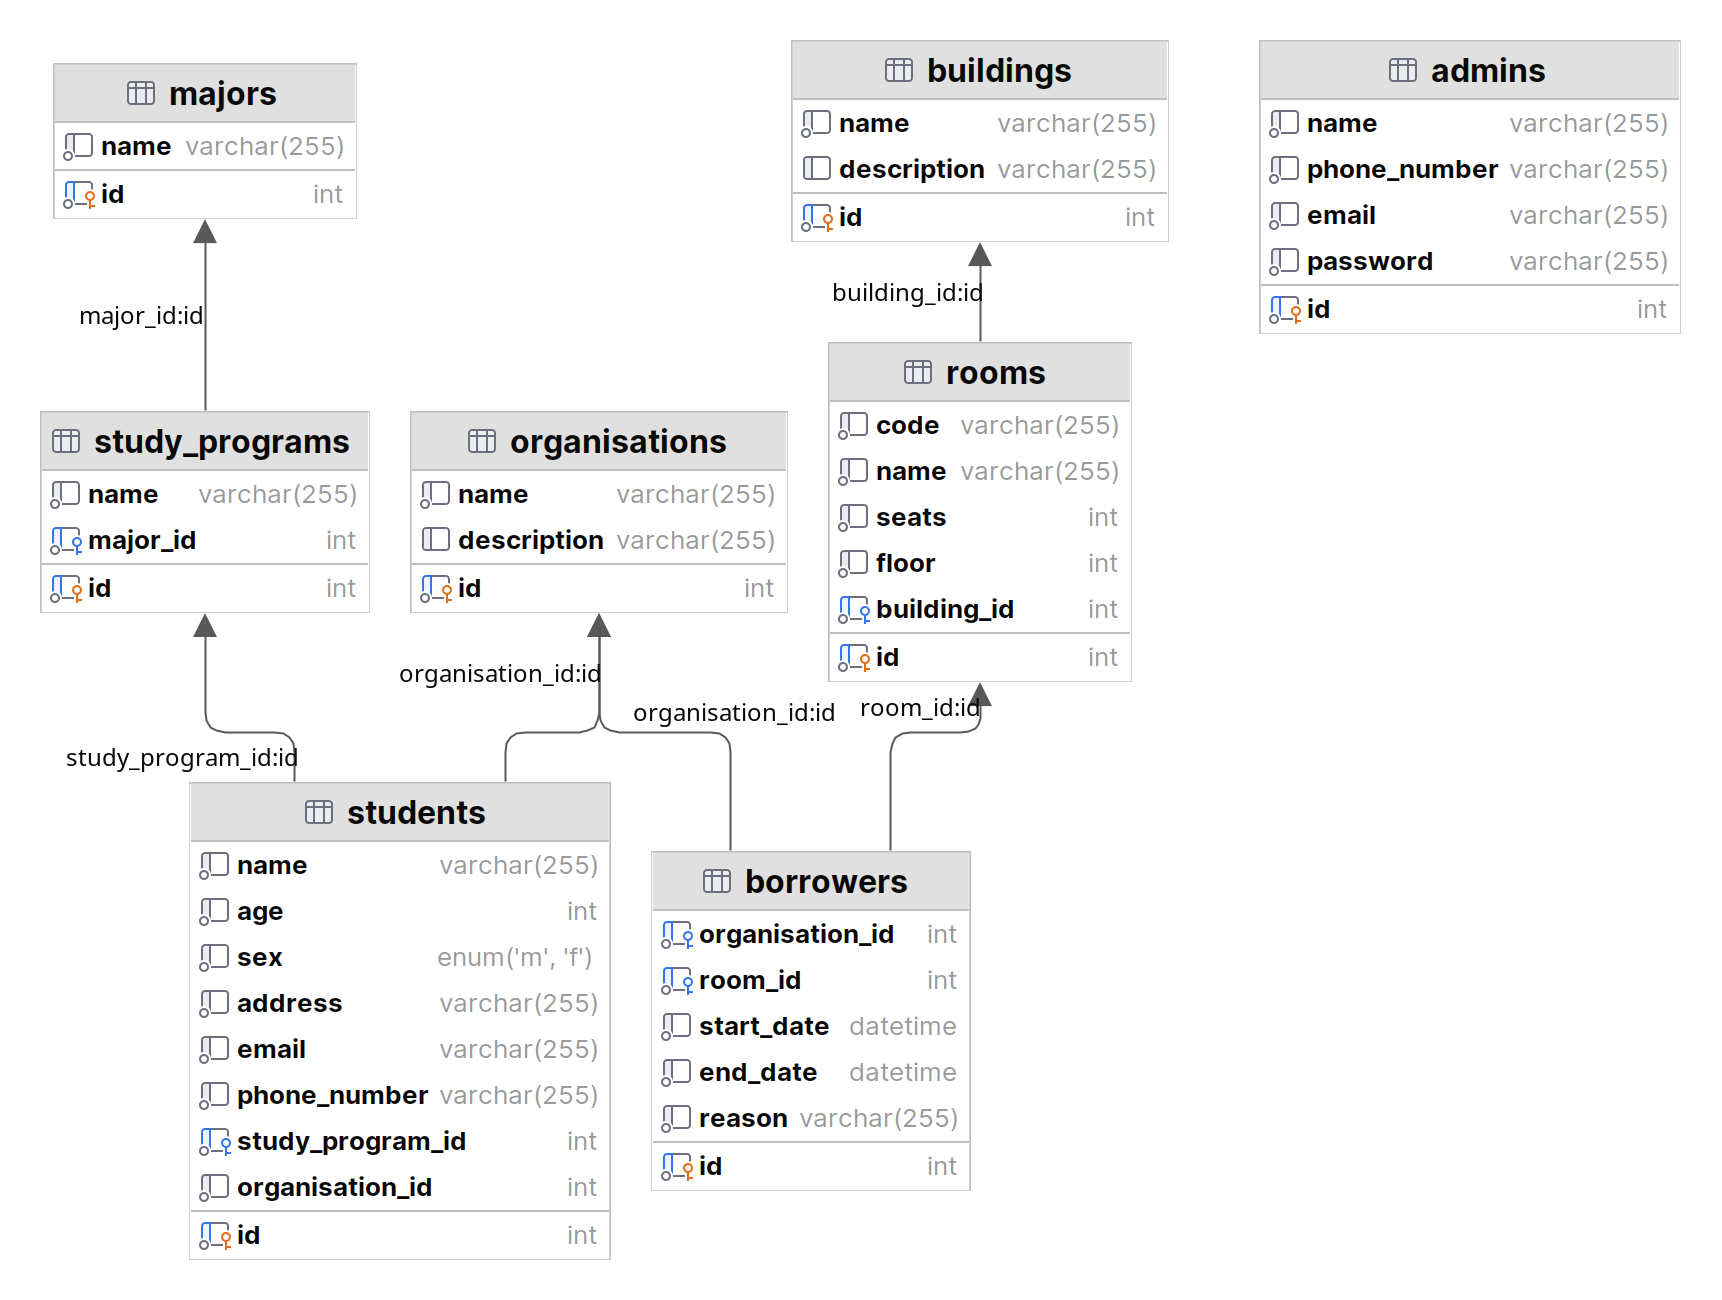
\includegraphics[width=\textwidth]{./images/rts-erd.png}
    \caption{Entity Relationship Diagram of the Room Tenant System}
\end{figure}

\pagebreak

\section{Database Schema}
The database schema are created using Data Definition Language in SQL. 
The schema is created to be compatible with MySQL 8.0.

\subsection{Admins Table}
This table is used to store the data for the admin who will manage the room tenant system in the application.
They are the ones who are responsible to review then approve or decline requests.

\begin{minted}[autogobble,fontsize=\small]{sql}
    CREATE TABLE `admins`
    (
        `id`           INT(11)      NOT NULL AUTO_INCREMENT PRIMARY KEY,
        `name`         VARCHAR(255) NOT NULL,
        `phone_number` VARCHAR(255) NOT NULL,
        `email`        VARCHAR(255) NOT NULL,
        `password`     VARCHAR(255) NOT NULL -- hashed with argon2 algorithm
        );
    \end{minted}
    
    \begin{figure}[h]
        \centering
        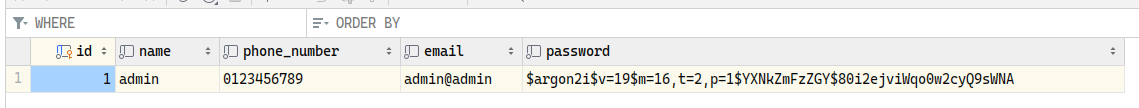
\includegraphics[width=\textwidth]{./images/admins-table.png}
        \caption{Admins table with data}
    \end{figure}

\subsection{Majors Table}
This table is used to store the data for the majors of the university.

\begin{minted}[autogobble,fontsize=\small]{sql}
    CREATE TABLE `majors`
(
    `id`   INT(11)      NOT NULL AUTO_INCREMENT PRIMARY KEY,
    `name` VARCHAR(255) NOT NULL
    );
\end{minted}

\begin{figure}[h]
    \centering
    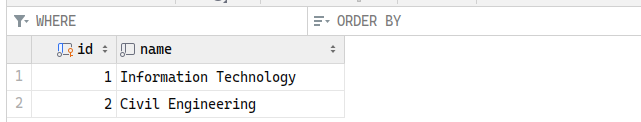
\includegraphics[width=.6\textwidth]{./images/majors-table.png}
    \caption{Majors table with data}
\end{figure}

\subsection{Study Programs Table}
This table is used to store the study programs that are available in the university.
Each study program will have a major attached to them.

\begin{minted}[autogobble,fontsize=\small]{sql}
    CREATE TABLE `study_programs`
    (
        `id`       INT(11)      NOT NULL AUTO_INCREMENT PRIMARY KEY,
        `name`     VARCHAR(255) NOT NULL,
        `major_id` INT(11)      NOT NULL
        );
    \end{minted}
    
    \begin{figure}[h]
        \centering
        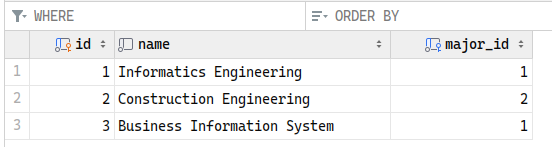
\includegraphics[width=.6\textwidth]{./images/study-programs-table.png}
        \caption{Study Programs table with data}
\end{figure}

\subsection{Students Table}
This table is used to store the data of the students. Each student stored in the room tenant system will have a study program
and an organisation.

\begin{minted}[autogobble,fontsize=\small]{sql}
    CREATE TABLE `students`
    (
        `id`               INT(11)         NOT NULL AUTO_INCREMENT PRIMARY KEY,
        `nim`              VARCHAR(255)    NOT NULL,
        `name`             VARCHAR(255)    NOT NULL,
        `age`              INT(11)         NOT NULL,
        `sex`              ENUM ('M', 'F') NOT NULL,
        `address`          VARCHAR(255)    NOT NULL,
        `email`            VARCHAR(255)    NOT NULL,
        `phone_number`     VARCHAR(255)    NOT NULL,
        `study_program_id` INT(11)         NOT NULL
        );
    \end{minted}

\begin{figure}[h]
    \centering
    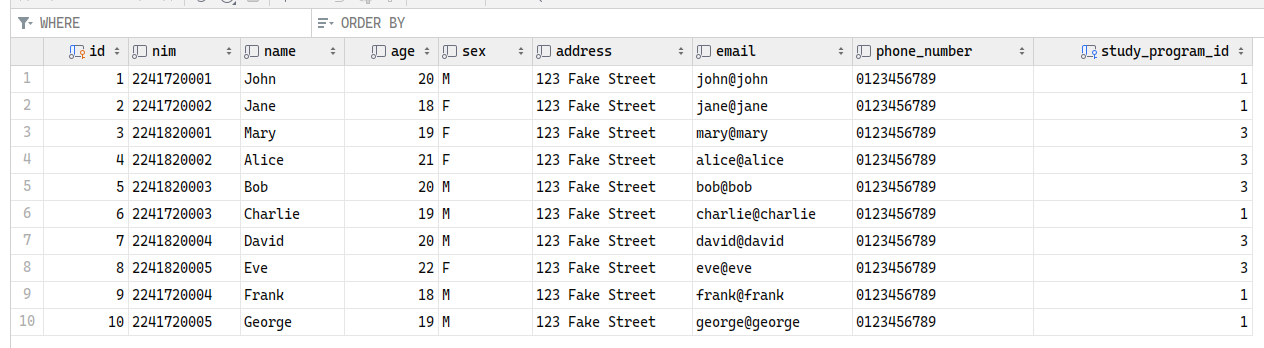
\includegraphics[width=\textwidth]{./images/students-table.png}
    \caption{Students table with data}
\end{figure}

\pagebreak

\subsection{Organisations Table}
This table is used to store the data for the student's organisation. 
Only an organisation can submit a request to borrow a room.

\begin{minted}[autogobble,fontsize=\small]{sql}
    CREATE TABLE `organisations`
    (
        `id`          INT(11)      NOT NULL AUTO_INCREMENT PRIMARY KEY,
        `name`        VARCHAR(255) NOT NULL,
        `description` VARCHAR(255)
        );
    \end{minted}
    
    \begin{figure}[h]
        \centering
        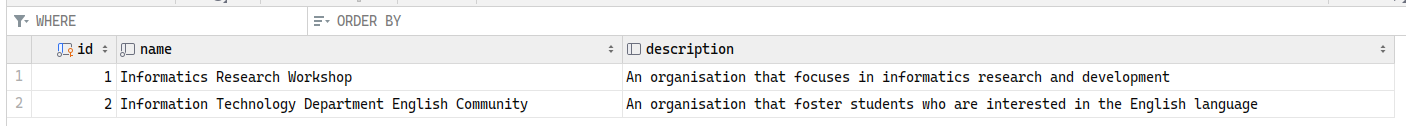
\includegraphics[width=\textwidth]{./images/organisations-table.png}
    \caption{Organisations table with data}
\end{figure}

\subsection{Students Organisations Table}
This table act as a pivot table that connects the many to many relationship between the student and an organisation.
Many to many is used because a single student can join multiple organisations and a single organisations can have multiple student members.

\begin{minted}[autogobble,fontsize=\small]{sql}
    CREATE TABLE `students_organisations`
    (
        `id`              INT(11) NOT NULL AUTO_INCREMENT PRIMARY KEY,
        `student_id`      INT(11) NOT NULL,
        `organisation_id` INT(11) NOT NULL
);
\end{minted}

\begin{figure}[h]
    \centering
    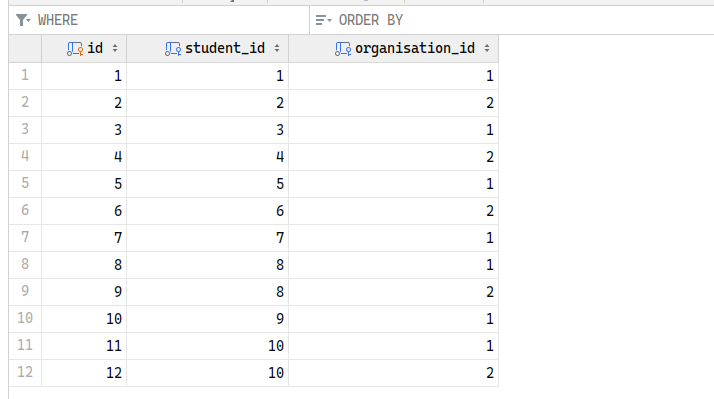
\includegraphics[width=\textwidth]{./images/students-organisations-table.png}
    \caption{Students Organisations table with data}
\end{figure}

\subsection{Buildings Table}
\begin{minted}[autogobble,fontsize=\small]{sql}
    CREATE TABLE `buildings`
    (
        `id`          INT(11)      NOT NULL AUTO_INCREMENT PRIMARY KEY,
        `name`        VARCHAR(255) NOT NULL,
        `description` VARCHAR(255)
        );
    \end{minted}
    
    \begin{figure}[h]
        \centering
        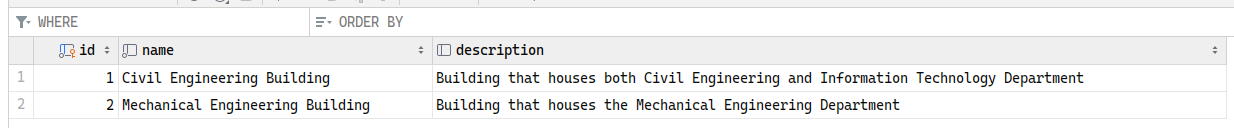
\includegraphics[width=\textwidth]{./images/buildings-table.png}
        \caption{Buildings table with data}
    \end{figure}
    
    \pagebreak
    
    \subsection{Rooms Table}
    \begin{minted}[autogobble,fontsize=\small]{sql}
        CREATE TABLE `rooms`
        (
            `id`          INT(11)      NOT NULL AUTO_INCREMENT PRIMARY KEY,
            `code`        VARCHAR(255) NOT NULL,
            `name`        VARCHAR(255) NOT NULL,
            `seats`       INT(11)      NOT NULL,
            `floor`       INT(11)      NOT NULL,
            `building_id` INT(11)      NOT NULL
            );
        \end{minted}
        
        \begin{figure}[h]
            \centering
            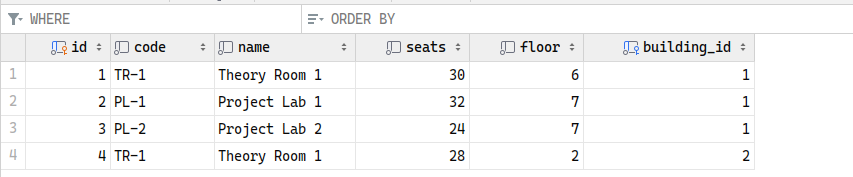
\includegraphics[width=\textwidth]{./images/rooms-table.png}
            \caption{Rooms table with data}
        \end{figure}
        
        \subsection{Borrowed Rooms Table}
        This table is used to store all of the borrowed rooms. 
        A student can represent an organisation and request a room which will then get reviewed and approved or rejected by the admin.
        
        \begin{minted}[autogobble,fontsize=\footnotesize]{sql}
            CREATE TABLE `borrowed_rooms`
            (
                `id`              INT(11)                                 NOT NULL AUTO_INCREMENT PRIMARY KEY,
                `student_id`      INT(11)                                 NOT NULL,
                `organisation_id` INT(11)                                 NOT NULL,
                `room_id`         INT(11)                                 NOT NULL,
                `start_date`      DATETIME                                NOT NULL,
                `end_date`        DATETIME                                NOT NULL,
                `reason`          VARCHAR(255)                            NOT NULL,
                `status`          ENUM('PENDING', 'APPROVED', 'REJECTED') NOT NULL,
                `approved_by`     INT(11)                                 NULL,
                `requested_at`    DATETIME                                NOT NULL
                );
            \end{minted}
            
            \pagebreak
            
            \begin{figure}[h]
    \centering
    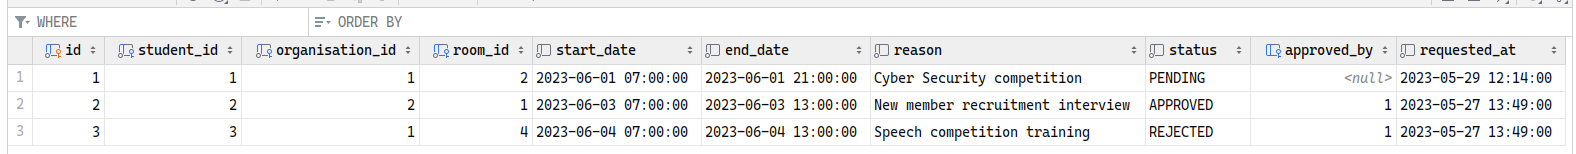
\includegraphics[width=\textwidth]{./images/borrowed-rooms-table.png}
    \caption{Borrowed Rooms table with data}
\end{figure}

\subsection{Table Constraints}
These are the constraints that is attached to each table. This process uses the \texttt{ALTER TABLE} command
to add a foreign key to the respective tables. This process is done last to make it more flexible when adding a constraint
since both table need to be exists before we can attach the constraint.

\begin{minted}[autogobble,fontsize=\small]{sql}
    ALTER TABLE `students`
    ADD FOREIGN KEY (`study_program_id`) REFERENCES `study_programs` (`id`);
ALTER TABLE `study_programs`
    ADD FOREIGN KEY (`major_id`) REFERENCES `majors` (`id`);
ALTER TABLE `students_organisations`
    ADD FOREIGN KEY (`student_id`) REFERENCES `students` (`id`);
ALTER TABLE `students_organisations`
    ADD FOREIGN KEY (`organisation_id`) REFERENCES `organisations` (`id`);
ALTER TABLE `borrowed_rooms`
    ADD FOREIGN KEY (`organisation_id`) REFERENCES `organisations` (`id`);
ALTER TABLE `borrowed_rooms`
    ADD FOREIGN KEY (`room_id`) REFERENCES `rooms` (`id`);
ALTER TABLE `borrowed_rooms`
    ADD FOREIGN KEY (`student_id`) REFERENCES `students` (`id`);
ALTER TABLE `borrowed_rooms`
    ADD FOREIGN KEY (`approved_by`) REFERENCES `admins` (`id`);
ALTER TABLE `rooms`
    ADD FOREIGN KEY (`building_id`) REFERENCES `buildings` (`id`);
\end{minted}

\pagebreak

\section{Populating Data}
As it stands currently, the database is empty. This section contains the query used to populate the database
using dummy data to simulate a real case scenario. This process is also known as \textit{data seeding}.

\begin{minted}[autogobble,fontsize=\scriptsize]{sql}
INSERT INTO `admins` (`id`, `name`, `phone_number`, `email`, `password`)
-- real value: `password`, hash salt: `asdfasdf`, algorithm: argon2
VALUES (1, 'admin', '0123456789', 'admin@admin', '$argon2i$v=19$m=16,t=2,p=1$YXNkZmFzZGY$80i2ejviWqo0w2cyQ9sWNA');

INSERT INTO `majors` (`id`, `name`)
VALUES (1, 'Information Technology'),
       (2, 'Civil Engineering');

INSERT INTO `study_programs` (`id`, `name`, `major_id`)
VALUES (1, 'Informatics Engineering', 1),
       (2, 'Construction Engineering', 2),
       (3, 'Business Information System', 1);

INSERT INTO `organisations` (`id`, `name`, `description`)
VALUES (1, 'Informatics Research Workshop', 'An organisation that focuses in informatics research and development'),
       (2, 'Information Technology Department English Community',
       'An organisation that foster students who are interested in the English language');

INSERT INTO `students` (id, nim, name, age, sex, address, email, phone_number, study_program_id)
VALUES (1, '2241720001', 'John', 20, 'M', '123 Fake Street', 'john@john', '0123456789', 1),
       (2, '2241720002', 'Jane', 18, 'F', '123 Fake Street', 'jane@jane', '0123456789', 1),
       (3, '2241820001', 'Mary', 19, 'F', '123 Fake Street', 'mary@mary', '0123456789', 3),
       (4, '2241820002', 'Alice', 21, 'F', '123 Fake Street', 'alice@alice', '0123456789', 3),
       (5, '2241820003', 'Bob', 20, 'M', '123 Fake Street', 'bob@bob', '0123456789', 3),
       (6, '2241720003', 'Charlie', 19, 'M', '123 Fake Street', 'charlie@charlie', '0123456789', 1),
       (7, '2241820004', 'David', 20, 'M', '123 Fake Street', 'david@david', '0123456789', 3),
       (8, '2241820005', 'Eve', 22, 'F', '123 Fake Street', 'eve@eve', '0123456789', 3),
       (9, '2241720004', 'Frank', 18, 'M', '123 Fake Street', 'frank@frank', '0123456789', 1),
       (10, '2241720005', 'George', 19, 'M', '123 Fake Street', 'george@george', '0123456789', 1);

INSERT INTO `students_organisations` (id, student_id, organisation_id)
VALUES (1, 1, 1),
       (2, 2, 2),
       (3, 3, 1),
       (4, 4, 2),
       (5, 5, 1),
       (6, 6, 2),
       (7, 7, 1),
       (8, 8, 1),
       (9, 8, 2),
       (10, 9, 1),
       (11, 10, 1),
       (12, 10, 2);

INSERT INTO `buildings` (`id`, `name`, `description`)
VALUES (1, 'Civil Engineering Building',
        'Building that houses both Civil Engineering and Information Technology Department'),
       (2, 'Mechanical Engineering Building', 'Building that houses the Mechanical Engineering Department');

INSERT INTO `rooms` (`id`, `code`, `name`, `seats`, `floor`, `building_id`)
VALUES (1, 'TR-1', 'Theory Room 1', 30, 6, 1),
       (2, 'PL-1', 'Project Lab 1', 32, 7, 1),
       (3, 'PL-2', 'Project Lab 2', 24, 7, 1),
       (4, 'TR-1', 'Theory Room 1', 28, 2, 2);

INSERT INTO `borrowed_rooms` (id, student_id, organisation_id, room_id, start_date, end_date, reason, approved_by,
                              status, requested_at)
VALUES (1, 1, 1, 2, '2023-06-01 07:00:00', '2023-06-01 21:00:00', 'Cyber Security competition', NULL, 'PENDING',
        '2023-05-29 12:14:00'),
       (2, 2, 2, 1, '2023-06-03 07:00:00', '2023-06-03 13:00:00', 'New member recruitment interview', 1, 'APPROVED',
        '2023-05-27 13:49:00'),
       (3, 3, 1, 4, '2023-06-04 07:00:00', '2023-06-04 13:00:00', 'Speech competition training', 1, 'REJECTED',
        '2023-05-27 13:49:00');
\end{minted}

\pagebreak

\section{Queries}
These are some examples of the queries that might be used on the application.

\subsection{Students Related Operations}
\begin{itemize}
    \item {
        Get all students along with their major, study program, and organisation

        \begin{minted}[autogobble,fontsize=\small]{sql}
            SELECT nim,
                   std.name,
                   age,
                   sex,
                   address,
                   email,
                   phone_number,
                   sp.name  AS study_program,
                   m.name   AS major,
                   org.name AS organisation
            FROM students_organisations std_org
                    JOIN students std ON std_org.student_id = std.id
                    JOIN organisations org ON std_org.organisation_id = org.id
                    JOIN study_programs sp ON std.study_program_id = sp.id
                    JOIN majors m ON sp.major_id = m.id;
        \end{minted}

        \begin{figure}[h]
            \centering
            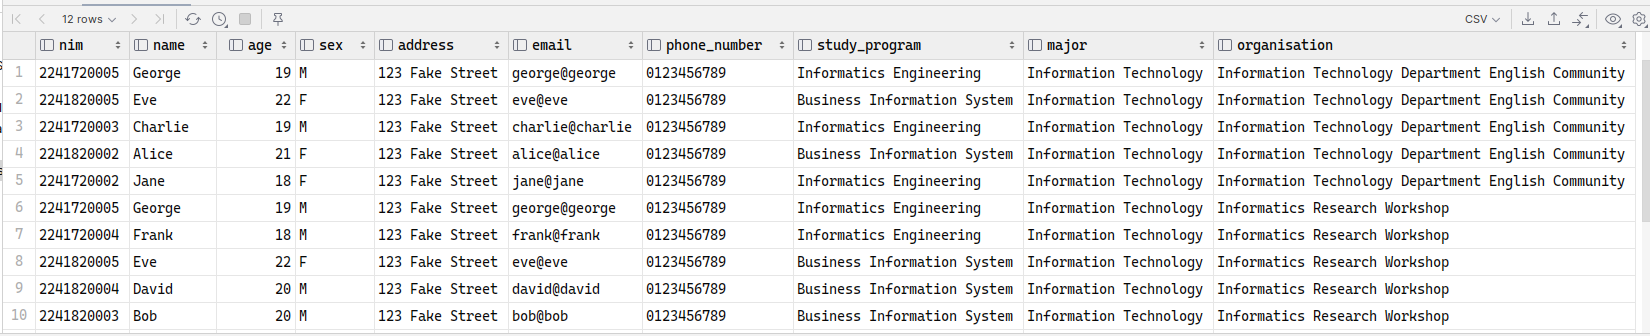
\includegraphics[width=\textwidth]{images/all-students-query.png}
            \caption{All students query result}
        \end{figure}
    }
    \pagebreak
    \item {
        Get all students from Informatics Engineering

        \begin{minted}[autogobble,fontsize=\small]{sql}
            SELECT nim,
                   std.name,
                   age,
                   sex,
                   address,
                   email,
                   phone_number,
                   sp.name AS study_program
            FROM students std
                    JOIN study_programs sp ON std.study_program_id = sp.id
            WHERE sp.name = 'Informatics Engineering';
        \end{minted}

        \begin{figure}[h]
            \centering
            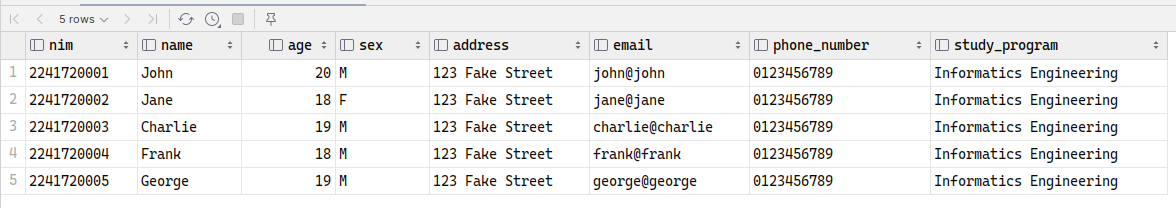
\includegraphics[width=\textwidth]{images/all-if-students-query.png}
            \caption{All informatics engineering students query result}
        \end{figure}
    }
    \item {
        Get all students who requested a room

        \begin{minted}[autogobble,fontsize=\small]{sql}
            SELECT nim,
                   std.name,
                   r.name    AS room,
                   r.floor   AS floor,
                   b.name    AS building,
                   br.status AS status,
                   br.reason AS reason
            FROM borrowed_rooms br
                    JOIN students std ON br.student_id = std.id
                    JOIN rooms r ON br.room_id = r.id
                    JOIN buildings b ON r.building_id = b.id;
        \end{minted}

        \begin{figure}[h]
            \centering
            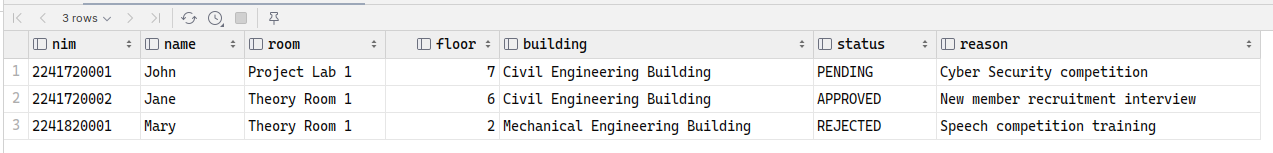
\includegraphics[width=\textwidth]{images/all-borrowing-students-query.png}
            \caption{All borrowing students query result}
        \end{figure}
    }
\end{itemize}

\pagebreak

\subsection{Rooms Related Operations}
\begin{itemize}
    \item {
        Get all rooms available for borrowing

        \begin{minted}[autogobble,fontsize=\small]{sql}
            SELECT r.name,
                   description,
                   floor,
                   b.name as building
            FROM rooms r
                    JOIN buildings b on r.building_id = b.id;
        \end{minted}

        \begin{figure}[h]
            \centering
            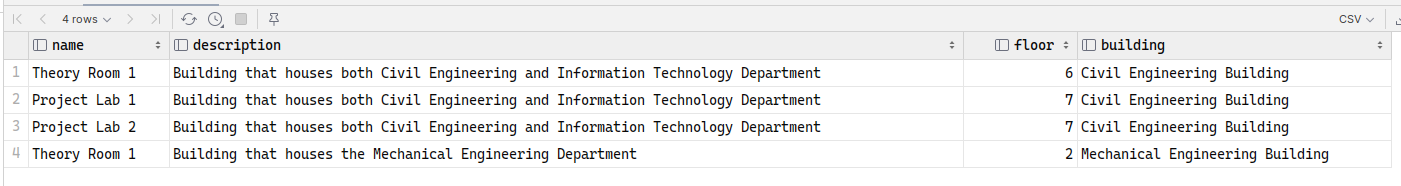
\includegraphics[width=\textwidth]{images/all-rooms-query.png}
            \caption{All rooms query result}
        \end{figure}
    }
    \item {
        Get all rooms in the 7th floor

        \begin{minted}[autogobble,fontsize=\small]{sql}
            SELECT r.name,
                   description,
                   floor,
                   b.name as building
            FROM rooms r
                    JOIN buildings b on r.building_id = b.id
            WHERE floor = 7;
        \end{minted}

        \begin{figure}[h]
            \centering
            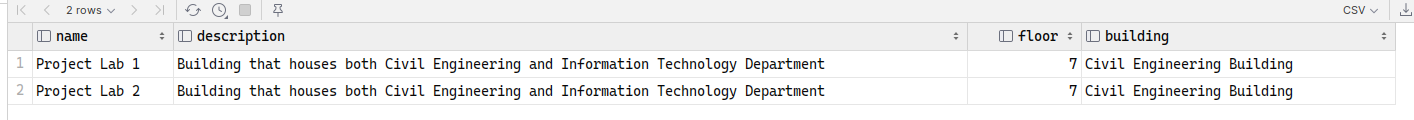
\includegraphics[width=\textwidth]{images/7th-floor-query.png}
            \caption{All rooms in 7th floor}
        \end{figure}
    }
\end{itemize}

\pagebreak

\section{Documentation}

\begin{figure}[h]
    \centering
    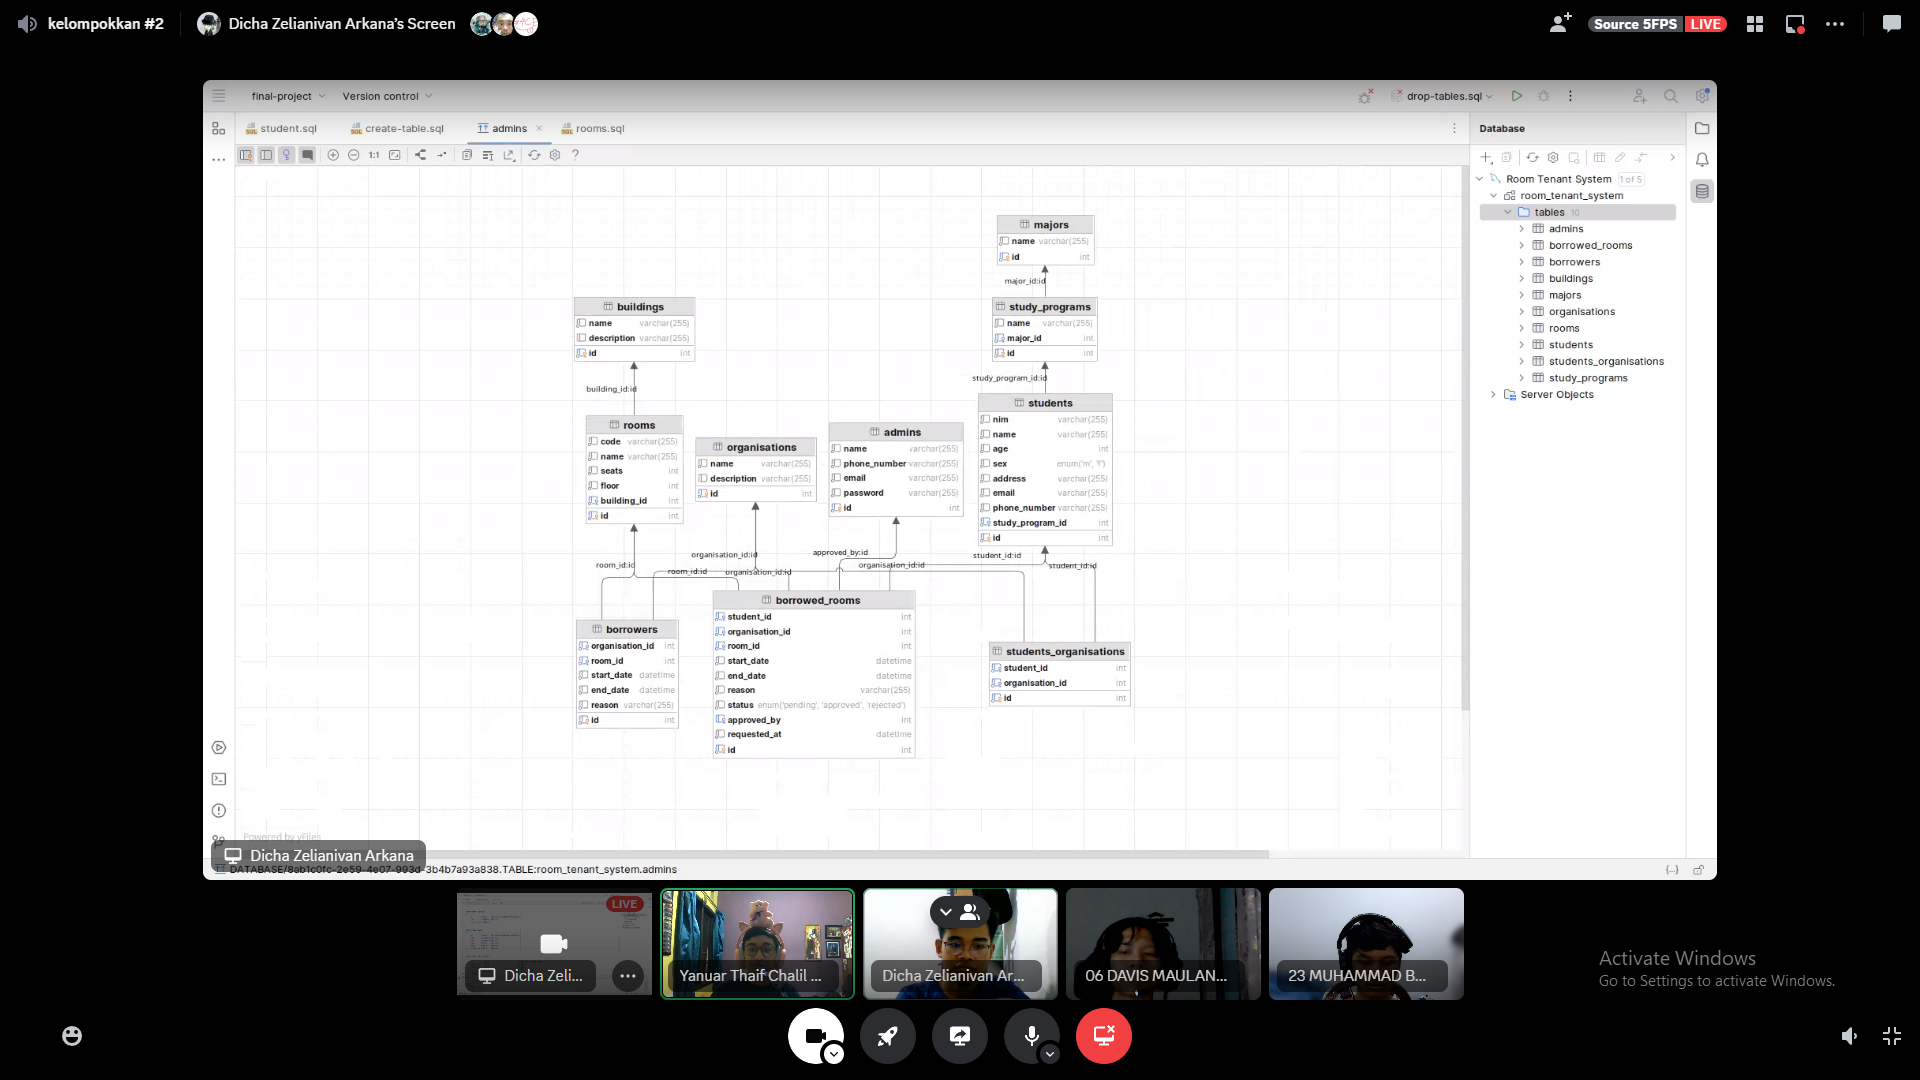
\includegraphics[width=.8\textwidth]{./images/documentation-1.png}
    \caption{Group ERD Discussion}
\end{figure}

\begin{figure}[h]
    \centering
    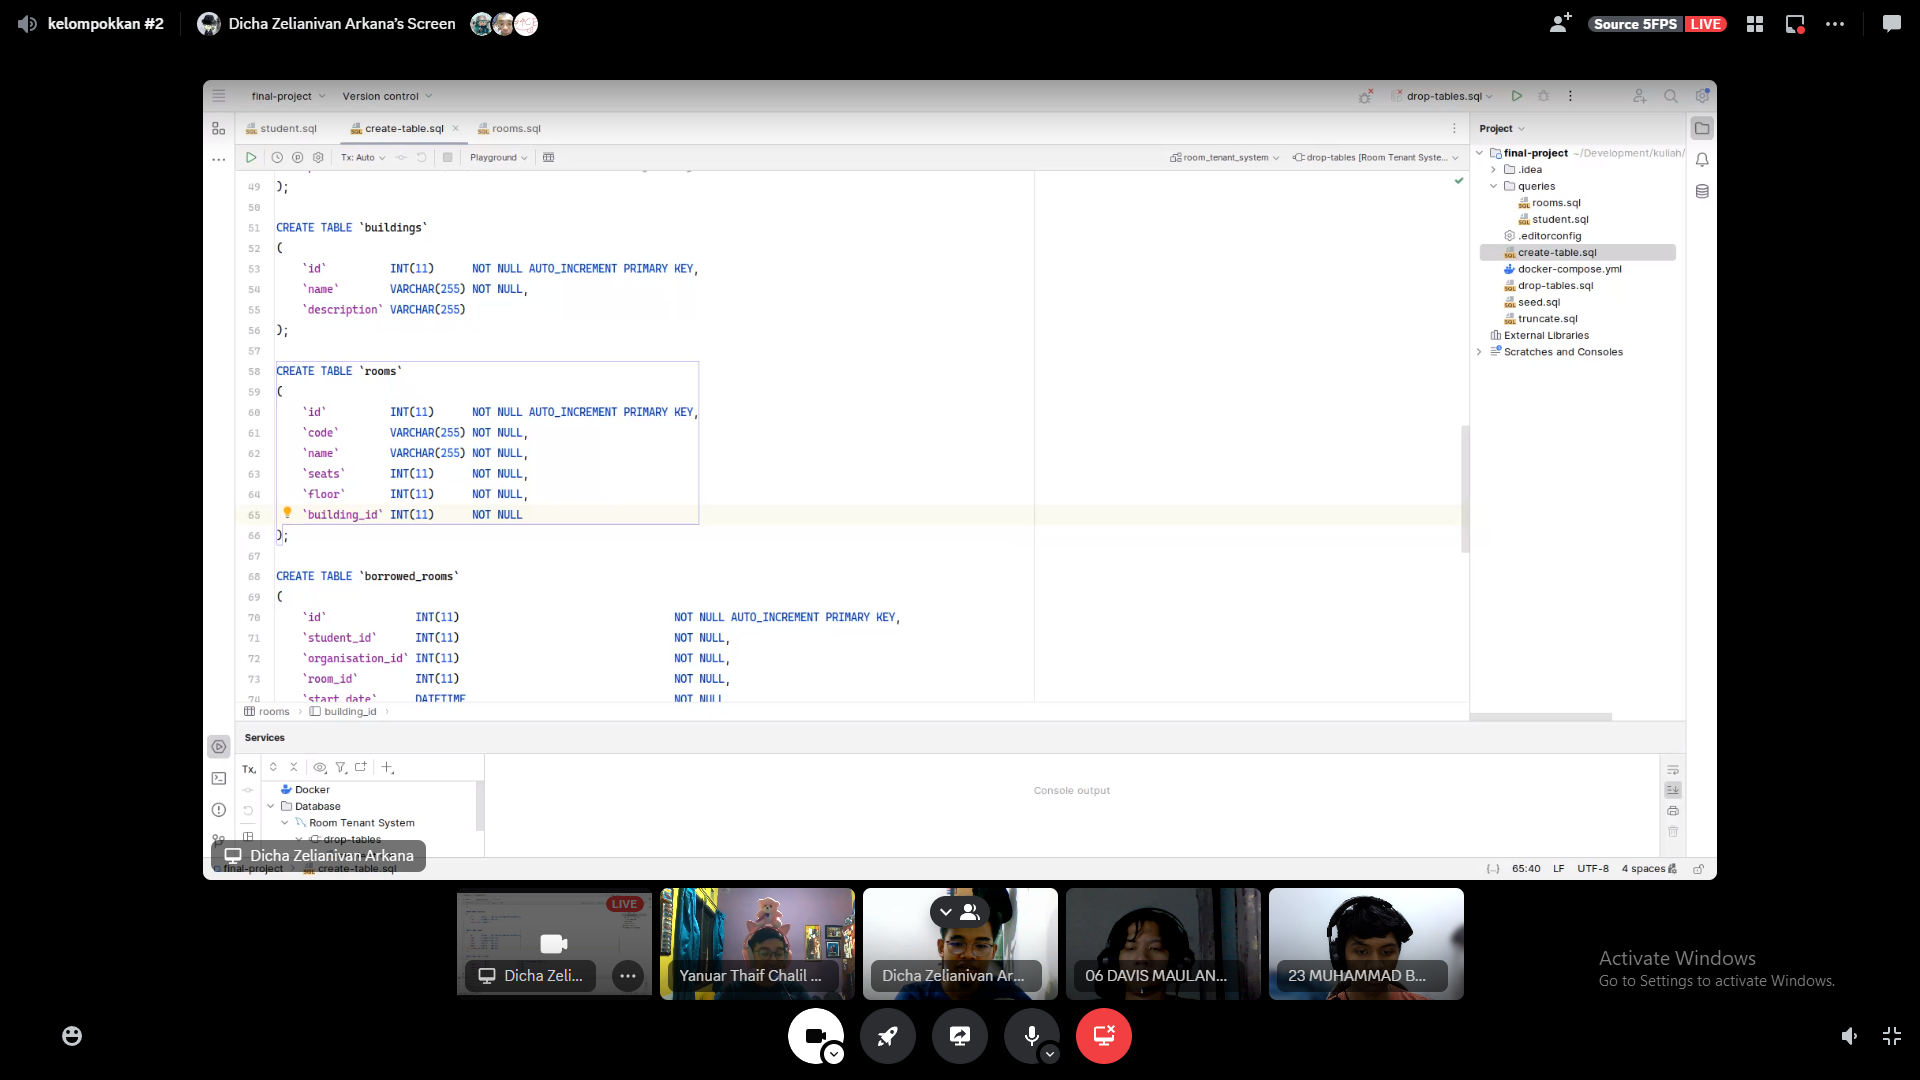
\includegraphics[width=.8\textwidth]{./images/documentation-2.png}
    \caption{Group Database Schema Discussion}
\end{figure}

\end{document}

